
\chapter{Queue and Stack}
\label{cha:queue-stack}

\section{Queue}
\label{sec:queue}

Queue is first in first out data structure.
In a FIFO data structure, the first element added to the queue will be processed first.
It is like an array, but the elements can be put into the queue at the end ant put out of the queue at the front.
As show in Figure \ref{fig:queue}.
\begin{figure}[!ht]
  \centering
  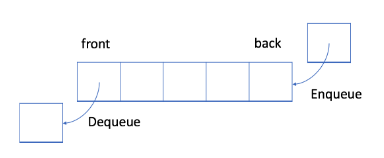
\includegraphics[width=0.8\textwidth]{queue.png}
  \caption{Queue}
  \label{fig:queue}
\end{figure}

There are two operations:
\begin{itemize}
\item enqueue: insert a new element at the end of the queue
\item dequeue: remove the element at the front(head) of the queue
\end{itemize}




\subsection{Queue and BFS}
\label{sec:queue-bfs}

Queue is usually used in BFS (Breadth-first Search).

Here is a simple template (Python):
\lstset{language=Python}
\begin{lstlisting}
  def BFS(root, target) -> int:
    queue = []
    step = 0
    queue.append(root)
    while queue:
        for node in queue:
            if node == target:
                return step
            # Add all node neighbors into the queue
            for neighbor in node.neighbors:
                queue.append(neighbor)
            queue.pop(0)
        step += 1
    # There is no path from root to target.
    return -1

\end{lstlisting}

\section{Stack}
\label{sec:stack}

Stack is last in first out data structure.
In a LIFO structure, the newest element added to the queue will be processed first.
It is like an array, but the elements can be put into the stack and put out of the queue at the end.
As show in Figure \ref{fig:stack}
\begin{figure}[!ht]
  \centering
  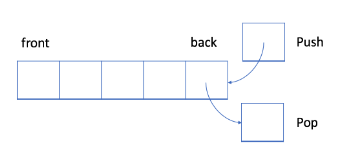
\includegraphics[width=0.8\textwidth]{stack.png}
  \caption{Stack}
  \label{fig:stack}
\end{figure}


There are two operations:
\begin{itemize}
\item push: add a new element at the end(top) of the stack
\item pop: remove the element at the end(top) of the stack
\end{itemize}

\subsection{Stack and DFS}
\label{sec:stack-dfs}

In most cases, we can also use DFS when using BFS. But there is an important difference: the traversal order.
Different from BFS, the nodes you visit earlier might not be the nodes which are closer to the root node.
As a result, the first path you found in DFS might not be the shortest path.

Here is a simple template (Python):
\lstset{language=Python}
\begin{lstlisting}
  def DFS(cur, target, visited: set) -> bool:
    if cur == target:
        return True
    for nei in cur.neighbors:
        if nei not in visited:
            visited.add(nei)
        if DFS(nei, target, visited):
            return True
    return False
\end{lstlisting}


The advantage of the recursion solution is that it is easier to implement.
However, there is a huge disadvantage: if the depth of recursion is too high, you will suffer from stack overflow.
In that case, you might want to use BFS instead or implement DFS using an explicit stack.

\section{Examples}
\label{sec:examples-2}

Here are some example on \href{https://github.com/mingmingli916/algorithms/tree/main/queque_and_stack}{Github}.



  


%%% Local Variables:
%%% mode: latex
%%% TeX-master: "algorithms"
%%% End:
